\problemname{Travar med böcker}

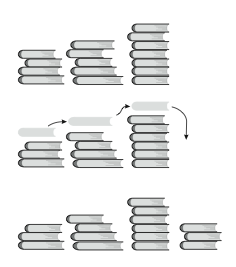
\includegraphics{Travar.png}

På ett bord ligger att antal travar med böcker. Varje dag tas en bok från varje trave. Dessa böcker bildar tillsammans en ny trave till höger om de andra, se figur 1. Om en trave blir tom skjuts travarna samman från höger. Eftersom det finns ett ändligt antal böcker, kommer förr eller senare samma upplägg att återkomma. Din uppgift blir nu att skriva ett program som frågar efter första uppläggets utseende och sedan tar reda på hur lång tid det tar innan ett upplägg som tidigare funnits, återkommer.

\begin{tabular}{|c|c|c|c|c|c|c|}
\hline
Dag&Hög 1&Hög 2&Hög 3&Hög 4&Hög 5&Hög 6\\\hline
1&4&5&7&&&\\
2&3&4&6&3&&\\
3&2&3&5&2&4&\\
4&1&2&4&1&3&5\\
5&1&3&2&4&6&\\
6&2&1&3&5&5&\\
7&\textbf{1}&\textbf{2}&\textbf{4}&\textbf{4}&\textbf{5}&\\
8&1&3&3&4&5&\\
9&2&2&3&4&5&\\
10&1&1&2&3&4&5\\
11&1&2&3&4&6&\\
12&1&2&3&5&5&\\
13&\textbf{1}&\textbf{2}&\textbf{4}&\textbf{4}&\textbf{5}&\\\hline
\end{tabular}

I tabellen ovan visas hur antalet böcker i travarna varierar under 13 dagar. I de kommande testerna är antalet böcker $ \le 50$, antalet travar som mest $ \le 15$ och antalet dagar $ \le 100$.

\section*{Indata}
Första raden består av ett heltal - antalet boktravar $N$.
Nästa rad består av $N$ heltal - antalet böcker i travarna

\section*{Utdata}
Utdata ska bestå av två heltal - de två första dagarna där uppställningen upprepades. Den första dagen ska skrivas ut först.


\section*{Poängsättning}
Din lösning kommer att testas på flera testfall. För att få 100 poäng så måste du klara alla testfall.

